%=========================================================================
% (c) Radim Loskot, 2014

\chapter{Úvod}
\label{Chapter.Introducion}

Funkci a význam webových prohlížečů netřeba dlouze představovat. Prohlížeče nám denně umožňují rychle a pohodlně procházet webový obsah a tzv. HTML dokumenty. HTML dokumenty nemusí být výhradně umístěny pouze na webu a na vzdálených úložištích, ale mohou přicházet i v rámci elektronické pošty nebo být součástí aplikační nápovědy, aj. Pro zobrazování HTML dokumentů používáme HTML zobrazovacích strojů. Jedním takovým strojem je CSSBox.

CSSBox je projekt experimentálního (X)HTML/CSS zobrazovacího stroje napsaného v~čistém jazyce Java. Projekt se snaží vyplnit prostor v implementacích zobrazovacích strojů v Javě, jejichž vývoj většinou ustal. Hlavním cílem projektu je poskytnout úplné a dále zpracovatelné informace o rozložení dokumentu. Vyjma analyzování dokumentu umožnuje již v samotném základu vizualizovat dokument jako prostý obrázek. V rámci samostatného podprojektu SwingBox dále díky komponentě \texttt{BrowserPane} přidává pokročilé grafické rozhraní pro zobrazování dokumentu, které dokáže reagovat i na události od uživatele.

V současné době CSSBox implementuje (X)HTML/CSS 2.1 analyzátor a výše zmíněné zobrazovací komponenty. Cílem této práce je projekt CSSBox rozšířit o možnost skriptování v dokumentu a implementovat vybranou základní množinu skriptovacího jazyka JavaScript. Jakým způsobem bude integrace docíleno, je popsáno v následujícím dokumentu.

V úvodu tohoto dokumentu -- v kapitole \ref{Chapter.DependenciesAnalysis.ScriptsInHTML} se pojednává o způsobech, jakým mohou být vloženy skripty do HTML dokumentů, a je demonstrován referenční přístup pro přidání skriptování do dokumentů podle doporučené specifikace HTML 5. Základní architektura použitých závislostí -- projektu CSSBox a SwingBox je uvedena v kapitolách \ref{Chapter.DependenciesAnalysis.CSSBox} a \ref{Chapter.DependenciesAnalysis.SwingBox}.

Kapitola \ref{Chapter.JavaScriptInJavaAnalysis} je zaměřena na analýzu dostupných skriptovacích strojů v současnosti a rozbor jejich API. V rámci této kapitoly je představeno i standardní Java API, které lze pro skriptování v Javě využít.

V poslední kapitole návrhu -- kapitole \ref{Chapter.Design} je nastíněn základní abstraktní návrh celé integrace nového rozšíření do projektu SwingBox. Postupně jsou ukázány jednotlivé náležitosti, které bude zapotřebí vykonat, aby bylo možné integraci provést. V závěru \linebreak[4]dokumentu -- kapitole \ref{Chapter.Design.SwingBoxIntegration} je demonstrována „registrace“ samotného rozšíření do projektu SwingBox.


\chapter{Analýza použitých technik}
\label{Chapter.DependenciesAnalysis}

V rámci této práce se budeme zabývat integrací podpory skriptování v JavaScriptu ve stroji CSSBox. Abychom mohli provést návrh knihovny implementující rozšíření stroje CSSBox, je zapotřebí upřesnit, jak jsou skripty v HTML dokumentech reprezentovány, jak jsou vykonávány a do jakého rozhraní je budeme integrovat.

Problematikou skriptování v HTML dokumentech se zabývá kapitola \ref{Chapter.DependenciesAnalysis.ScriptsInHTML}. Na projekt CSSBox, jeho architekturu je zaměřena kapitola \ref{Chapter.DependenciesAnalysis.CSSBox}. Komponenta, která bude použita pro zobrazování HTML dokumentů a která bude implementovat rozšíření skriptování v těchto dokumentech, je popsána v kapitole \ref{Chapter.DependenciesAnalysis.SwingBox}. 

\section{Klientské skripty v HTML dokumentu}
\label{Chapter.DependenciesAnalysis.ScriptsInHTML}

Klientský skript je program, který může doprovázet HTML dokument nebo být do něj přímo vložen. Skript je vykonáván na straně klienta buď ihned po jeho načtení, nebo až poté, co je načten celý dokument. Skripty mohou:

\begin{itemize}
  \item sloužit k modifikaci obsahu dokumentu, jakmile je načten;
  \item být spuštěny událostmi ovládacích prvků;
  \item být využity pro validaci a odesílání obsahu formuláře na server.
\end{itemize}

\noindent Pro vložení skriptu do HTML dokumentu máme dva způsoby:

\begin{enumerate}
  \item Uvést skript v dokumentu ve speciální značce \texttt{<script>};
  \item Vložit skript do atributu události elementů, které podporují volání akcí. 
\end{enumerate}

Skripty ve značkách \texttt{<script>} jsou spouštěny samostatně a vždy bez závislosti na výskytu některé události. Při zpracovávání dokumentu jsou jednotlivé skripty v těch značkách vykonány. Jak a v jakém pořadí spouštění skriptů probíhá, popíšeme v této kapitole.

V rámci samotné značky \texttt{<script>} můžeme podle doporučené specifikace HTML 5 rozlišit celkem 6 atributů. Všechny atributy řídí vykonávání skriptu v určitém momentu jeho zpracovávání a jejich dynamická změna nemá žádný efekt na průběh skriptu. Specifikace uvádí následující atributy:

\begin{enumerate}
  \item \textbf{\texttt{src}} -- URL\footnote{URL (Uniform Resource Locator) -- řetězec sloužící k jednoznačné identifikaci zdroje} souboru s externím skriptem;
  \item \textbf{\texttt{type}} -- MIME\footnote{MIME (Multipurpose Internet Mail Extensions) -- internetový standard definující různé typy internetového média} typ skriptu;
  \item \textbf{\texttt{charset}} -- typ kódování souboru s externím skriptem;
  \item \textbf{\texttt{async}} -- udává, zda bude skript spuštěn asynchronně;
  \item \textbf{\texttt{defer}} -- specifikuje odložení spuštění skriptu až do dokončení načtení dokumentu;
  \item \textbf{\texttt{crossorigin}} -- specifikuje umístění zdroje skriptu při selhání načítání skriptu. 
\end{enumerate}

Kromě samotných atributů elementu skriptu specifikace HTML 5 doporučuje asociovat s elementem \texttt{<script>} i speciální příznaky. Příznaky jsou nastavovány na základě toho, kde byl element skriptu zpracován a na základě výše zmíněných atributů. Uvedenými příznaky ve specifikaci jsou:

\begin{enumerate}
  \item \textbf{\texttt{already-started}} -- značí, zda byl skript již vykonán. Při klonování elementu \texttt{<script>} se musí příznak sdílet;
  \item \textbf{\texttt{parser-inserted}} -- příznak je nastaven pro všechny skripty vložené do dokumentu HTML nebo XML parserem, např. při vložení pomocí \texttt{document.write()}. Skripty vložené při vytváření dokumentu nemají tento příznak nastaven;
  \item \textbf{\texttt{force-async}} -- během počátečního zpracování dokumentu je příznak nastaven. Skripty nemají tento příznak nastaven, pokud jsou vytvořeny a vloženy do dokumentu dodatečně, nebo pokud mají specifikovaný atribut \texttt{async};
  \item \textbf{\texttt{ready-to-be-parser-executed}} -- příznak používaný pouze pro skripty, které byly vloženy dodatečně některým z parserů dokumentu. Příznak je nastaven, pokud dojde k úspěšnému načtení skriptu z externího zdroje;
  \item \textbf{\texttt{script-type a script-charset}} -- jsou příznaky, které pouze reflektují atributy elementu \texttt{<script>}. Pokud nejsou atributy skriptu nastaveny, nebo jsou nastaveny špatně, pak obsahují tyto příznaky opravené nebo výchozí hodnoty těchto atributů.
\end{enumerate}

Nastavování části výše zmíněných příznaků by měl obsluhovat parser dokumentu během tvorby elementu \texttt{<script>}. Před spuštěním skriptu by se podle specifikace HTML 5 měla provést příprava skriptu. Příprava zahrnuje několik kroků, které nastaví příznaky např. \texttt{script-type} a \texttt{script-charset}, případně upraví příznaky nastavené parserem. 

Příprava elementu \texttt{<script>} pro jeho budoucí spuštění je provedena, pokud skript nemá nastaven příznak \texttt{parser-inserted} a pokud nastane:

\begin{enumerate}
  \item vložení elementu požadovaného skriptu do dokumentu,
  \item vložení nového uzlu nebo fragmentu dokumentu do již existujícího skriptu,
  \item nastavení atributu src, který nebyl předtím nastaven.
\end{enumerate}

Prvotní fáze přípravy skriptu, jíž výsledkem je nastavení příznaku \texttt{already-started}, tj., zda je skript spustitelný, je znázorněna v příloze \ref{Annex.ScriptPreprocessing}. Během přípravy dochází také k~zahájení načítání skriptů z externích zdrojů a umisťování jejich spuštění do front skriptů ke spuštění, aniž by docházelo k čekání, než jsou skripty kompletně načteny. 

Pokud spouštíme skript existující přímo v dokumentu, je jeho vykonávání zahájeno ihned a to i bez ohledu, zda předchozí skripty skončily své provádění. Všechny skripty, které mají uvedený externí zdroj, nejsou \texttt{parser-inserted} a byly již načteny, jsou spouštěny také okamžitě bez zbytečného čekání. Naopak problematika umísťování blokujících skriptů z důvodu čekání na zpracování stylů nebo \texttt{parser-inserted} skriptů do front skriptů ke spuštění je značně komplikovaná. Více o zpracovávání těchto skriptů si lze dočíst v samotné specifikaci HTML 5 \cite{Bibliography.HTML5.Scripting}.

\section{Renderovací stroj CSSBox}
\label{Chapter.DependenciesAnalysis.CSSBox}

CSSBox je projekt (X)HTML/CSS renderovacího stroje napsaného v čistém jazyce Java. Projekt klade velký důraz na poskytnutí informací o zpracovávané stránce.

Renderovací stroj CSSBox očekává na svém vstupu model dokumentu - DOM\footnote{DOM (Data Object Model) -- objektově orientovaná reprezentace XML nebo HTML dokumentu}. Dokument je v rámci stroje získáván pomocí parseru NekoHTML, ale může být získáván i jiným způsobem. Rozhraním pro všechny zdroje dokumentu je abstraktní třída \texttt{DOMSource}. Pro zpracování stylů dokumentu slouží třída \texttt{DOMAnalyzer}, která převede aktuální dokument na rozložení stránky. Výsledný model rozložení stránky se využívá pro zobrazení stránky, v knihovně je pro tento účel implementována komponenta \texttt{BrowserCanvas}.

\begin{figure}[H]
  \begin{center}
    \scalebox{0.65}{
      \includegraphics{fig/cssbox.pdf}
    }
    \caption{Hierarchie zobrazovacích komponent třídy \texttt{Box}}
    \label{Figure.BoxHierarchy}
  \end{center}
\end{figure}

Komponenta \texttt{BrowserCanvas} vytváří strom vykreslených objektů třídy Box. Strom je vytvářen ze vstupního dokumentu a výstupu analyzátoru stylů. Ke každému vykreslovanému elementu dokumentu, je vytvořen třídou \texttt{BrowserCanvas} jeho odpovídající \texttt{Box}. Každý prvek HTML stránky se pojí se specializovanou třídou \texttt{Box}, jak je znázorněno na obrázku \ref{Figure.BoxHierarchy}. Typ boxu nemusí být určen pouze typem elementu dokumentu, ale i jeho styly. Pokud blokový prvek má nastaveno zobrazení na řádku, tak bude ve stromu reprezentován třídou \texttt{InlineBox} a nikoliv třídou \texttt{BlockBox}. 

\clearpage

\section{Projekt SwingBox}
\label{Chapter.DependenciesAnalysis.SwingBox}

V rámci podprojektu SwingBox, který je součástí projektu CSSBox, byla vyvinuta komponenta \texttt{BrowserPane} \cite{Bibliography.SwingBox.Thesis}, která rozšiřuje funkčnost základního zobrazování dokumentu komponentou \texttt{BrowserCanvas}. Komponenta \texttt{BrowserPane} vychází ze třídy \texttt{JEditorPane}, ve které předefinovává výchozí zobrazování (X)HTML dokumentů. Pro zobrazování těchto dokumentů využívá třídu \texttt{SwingBoxEditorKit}, která zařizuje veškerou logiku zobrazování.

Komponenta \texttt{BrowserPane} umožňuje načítat dokumenty předáním jejich URL adresy, předáním dokumentu jako textový řetězec, nebo předání vstupního streamu s dokumentem. Na základě typu dokumentu, který má být zobrazen, komponenta dále volá pro čtení dokumentu odpovídající kit -- v našem případě \texttt{SwingBoxEditorKit}. Kit zařizuje s použitím třídy \texttt{ContentReader} načtení rozvržení stránky (viz kapitola \ref{Chapter.DependenciesAnalysis.CSSBox}) a jeho převod na reprezentaci dokumentu \texttt{SwingBoxDocument}, tak jak ho přijímá rozhraní komponenty \texttt{JEditorPane}. Třída \texttt{ContentReader} provádí převod rozvržení stránky na prvky dokumentu, tzn., převádí objekty třídy \texttt{Box} na objekty třídy \texttt{ElementSpec}. Veškeré načítání dokumentu ve formě DOM a jeho rozvržení třídou \texttt{DOMAnalyzer}, je prováděno ve třídě \texttt{CSSBoxAnalyzer}, na kterou je reference uvnitř třídy \texttt{ContentReader}.

\begin{figure}[H]
  \begin{center}
    \scalebox{0.70}{
      \includegraphics{fig/swingbox.pdf}
    }
    \caption{Diagram tříd komponenty \texttt{BrowserPane}}
    \label{Figure.SwingBoxDesign}
  \end{center}
\end{figure}

Prvky dokumentu \texttt{SwingBoxDocument}, které vytváří třída \texttt{ContentReader}, jsou vykreslovány na zobrazovací plochu \texttt{BrowserPane} ve formě pohledů \texttt{View}. Vykreslování řídí automaticky komponenta \texttt{JEditorPane}, která zná referenci na továrnu pohledů \linebreak\texttt{SwingBoxViewFactory}. Továrna pohledů je používaná komponentou \texttt{JEditorPane} vždy při potřebě vykreslit požadovaný dokument. Továrna se využívá pro vytváření pohledů pro každý prvek dokumentu \texttt{SwingBoxDocument}. Jelikož prvky dokumentu \texttt{ElementSpec} v~sobě zapouzdřují informaci o tom, jaký box obalují, je možno vytvořit pohledy, které přesně korespondují s množinou boxů uvedených v kapitole \ref{Chapter.DependenciesAnalysis.CSSBox}.

\chapter{Analýza podpory skriptování v~jazyce JavaScript v~Javě}
\label{Chapter.JavaScriptInJavaAnalysis}

Tato kapitola se zabývá analýzou skriptování a nástrojů, které lze využít pro tvorbu skriptů. Zaměřuje se na skriptovací jazyk JavaScript a jeho použití v~Javovských aplikacích. Kapitola záměrně popisuje zejména skriptovací stroj Rhino a standardní skriptovací Java API, jež lze pro skriptování použít.

Skriptovací jazyky jsou programovací jazyky, které nám umožňují psát tzv. skripty. Na rozdíl od kompilovatelných zdrojových kódů, je kód skriptu vyhodnocován a interpretován tzv. virtuálním strojem -- za běhu skriptu. Většina skriptovacích jazyků je typována dynamicky za běhu skriptu, což nám umožnuje vytvářet proměnné bez specifikace typu, neboť typová konverze je prováděna automaticky. V dynamických jazycích můžeme použít jednu proměnnou pro uložení více typů. Skriptovací jazyky mají jednoduchou syntaxi, což umožňuje v určitých případech vyřešit poměrně složité problémy pomocí relativně krátkého kódu, efektivně a poměrně v krátkém čase.

Ačkoliv jsou skripty obvykle kompilovány za běhu skriptu, lze je zkompilovat do mezikódu Javy a nechat je vykonat JVM\footnote{JVM  (Java Virtual Machine) -- virtuální stroj Javy zpracovávající mezikód jazyka Java (Java bytecode)}. V~Javě bylo implementováno mnoho skriptovacích Jazyků, využívajících různá rozhraní pro skriptování, což bylo mj. i důvodem pro vznik obecného skriptovacího Java API (viz kapitola \ref{Chapter.JavaScriptInJavaAnalysis.ScriptingJavaAPI}). Mezi nejrozšířenější skriptovací jazyky pro Javu můžeme zařadit BeanShell, s velmi podobnou syntaxí jakou disponuje Java, a další implementace již existujících jazyků v~Javě jako je např. Jython -- implementace Pythonu,  JRuby -- implementace Ruby, Groovy aj.

Interpretů JavaScriptu implementovaných v~Javě běžících na JVM není mnoho. Z důvodu výkonnosti je většina interpretů JavaScriptu pro webové prohlížeče napsána nativně v~C nebo C++ a využívá JIT\footnote{JIT (Just in Time) -- metoda překladu urychlující běh skriptu překladem kódu do strojového jazyka} techniky. Jmenovitě nejznámější nativní javasriptová jádra jsou z rodiny „Monkey“, kterou spravuje společnost Mozilla, a která jsou postupně využívána ve webovém prohlížeči Firefox. Dalšími jádry ostatních webových prohlížečů je V8 použité v Google Chrome, Carakan v Opeře, Chakra v Iternet Exploreru nebo JavaScriptCore v~prohlížeči Safari.

Nejvíce používané interprety cílené pro Java aplikace máme v současnosti pouze tři. Nejznámějším interpretem je již zmíněné Rhino (kapitola \ref{Chapter.JavaScriptInJavaAnalysis.Rhino}) \cite{Bibliography.Rhino.Docs}, které je i dodáváno v~Oracle implementaci JDK\footnote{JDK (Java Development Kit) -- balík základních nástrojů potřebných pro vývoj aplikací pro platformu Java} 6 a 7, kde realizuje výchozí skriptovací stroj pro Javu. Dalším interpretem s velkým budoucím potenciálem, který bude součásti Oracle implementace JDK 8 a který je stále ve vývoji, je interpret Nashorn \cite{Bibliography.Nashorn.Project} (kapitola \ref{Chapter.JavaScriptInJavaAnalysis.Nashorn}). Oba zmíněné skriptovací jazyky implementují standardní skriptovací Java API. Rhino bylo o skriptovací API rozšířeno firmou Sun, kdežto Nashorn je vyvíjen s tímto API zprvu počátku. Posledním a nepříliš používaným interpretem je YAJI \cite{Bibliography.YAJI.Project}, který se snaží oživit starý interpret FESI \cite{Bibliography.FESI.Project} tím, že do něho přidává většinu vlastností z nejnovější specifikace ECMAScriptu.

\section{Rhino}
\label{Chapter.JavaScriptInJavaAnalysis.Rhino}

Rhino je implementace javasriptového jádra napsaná v programovacím jazyce Java. Projekt Rhina byl zahájen v roce 1997 firmou Netscape, kdy firma potřebovala integrovat podporu JavaScriptu do budoucího prohlížeče založeném na platformě Java. Rhino vzniklo portem nativní knihovny SpiderMonkey, takže i nyní si lze v kódu nevšimnout Javovských ekvivalentů nepodmíněných skoků. \cite{Bibliography.Rhino.History}

Projekt prohlížeče, tzv. Javagatoru, byl ovšem brzy pozastaven a Rhino zůstalo dále jen velmi pozvolna vyvíjené několika vlastníky, včetně společnosti Sun. V roce 1998 bylo Rhino uvolněno společnosti Mozilla a držitelé licencí se dohodli, že vydají Rhino jako svobodný software. Nyní je Rhino spravováno společností Mozilla. \cite{Bibliography.Rhino.History}

\subsection{Vlastnosti Rhina}
\label{Chapter.JavaScriptInJavaAnalysis.Rhino.RhinoFeatures}

V současnosti je vydáno Rhino s označením 1.7R4. Nejnovější verze implementuje všechny vlastnosti Javasriptu 1.7, tzn. je plně ekvivalentní s 3. vydáním standardu \linebreak ECMA-262 ECMAScript a přidává některé nové vlastnosti, jako jsou doplňky pro práci s poli a podpora E4X\footnote{Rozšíření programovacího jazyka ECMAScript, které přidává podporu nativního XML a vychází z normy ECMA-357 ECMAScript pro XML.}. Od verze 1.7R3 Rhino přidává i částečnou podporu Javasriptu 1.8 a 5. vydání ECMAScriptu, která byla nejnovější verzí 1.7R4 zejména optimalizována a jen mírně rozšířena. \cite{Bibliography.Rhino.v17R3,Bibliography.Rhino.v17R4}

Významnou předností Rhina je jeho dobrá provázanost s Javou. Napojení na jazyk Java a umožnění hostování objektů Javy nám zpřístupňuje z kódu JavaScriptu používat téměř libovolný balíček a třídu z Javy. Výjimky pro třídy, které by neměly být zpřístupňěny jsou definované bezpečnostními politikami ve třídě \texttt{SecurityManager} (Java API) a dodatečně třídou \texttt{ClassShutter} (knihovna Rhino). Jamile je přístup do třídy povolen, lze z kódu JavaScriptu tuto třídu konstruovat, volat její libovolnou metodu či přistupovat k~atributům třídy. Aby bylo možné objekt Javy v JavaScriptu používat, musí vždy implementovat rozhraní \texttt{Scriptable} (viz kapitola \ref{Chapter.JavaScriptInJavaAnalysis.Rhino.ScriptingWithRhino}).V případě hostování jazyka Javy, je rozhraní \texttt{Scriptable} implementováno automaticky pomocí třídy \texttt{WrapFactory}. 

Mezi další přednosti Rhina patří možnost rozdělení skriptů do modulů, tak jak bylo specifikováno skupinou CommonJS\footnote{CommonJS -- Skupina lidí snažící se vytvořit jednotné JavaScriptového prostředí pro servery, desktopy a prohlížeče.} a možnost vysledovat zdroj odkud skript pochází a zpracovávat skript podle odpovídající bezpečnostní politiky. Bezpečnostní politiky v Rhinu vycházejí z Netscape Navigatoru a jejich aplikace je založená na kontrole URL zdroje. \cite{Bibliography.Rhino.Overview}

Rhino umožňuje dva režimy -- interaktivní a kompilovaný. V kompilovaném módu je kód přeložen do mezikódu Javy a interpretován dále v JVM. V interaktivním módu je skript spouštěn jednoduchým interpretem, aniž by docházelo ke generování mezikódu Javy.

Poslední zajimavou vlastností knihovny Rhino je poskytování z kódu JavaScriptu podpory pro implementaci rozhraní a abstraktních tříd Javy. Implementaci nedefinovaných metod z JavaScriptu zajišťuje třída objektového adaptéru \texttt{JavaAdapter}. Adaptér vytváří pomocí reflexe objekty Javy a implementuje do objektů navíc metody rozhraní \texttt{Scriptable}, čímž zpřístupňuje tyto objekty pro přímé použití ve skriptech JavaScriptu. Adaptér můžeme buď přímo zavolat nebo ho nechat Rhino automaticky odvodit. 

%\begin{table}[ht] 
%    \texttt{\begin{tabbing}
%      	{ }{ }{ }{ }{ }\={ }{ }\=\+\kill
%      	// přímé zavolání adaptéru \\
%      	\textbf{var} arr1 = \textbf{new} JavaAdapter(java.util.ArrayList, {}); \\
%		// automatické odvození -- Rhino zavolá adaptér automaticky \\
%		\textbf{var} arr2 = \textbf{new} java.util.ArrayList();
%    \end{tabbing}}
%\end{table}
%\vspace{-12mm}
%\begin{algoritmus}
%	\caption{Demonstrace explicitního a implicitního volání adaptéru Javy}
%	\label{Algorithm.JavaAdapterInRhino}
%\end{algoritmus}

\subsection{Skriptování s Rhinem}
\label{Chapter.JavaScriptInJavaAnalysis.Rhino.ScriptingWithRhino}

Zdrojové kódy Rhina jsou strukturovány do několika hlavních balíků. Pro konstrukci skriptů v~Javě využijeme hlavně veřejné API z balíku \texttt{org.mozilla.JavaScript}.

Základním prvkem pro spuštění jakéhokoliv skriptu je objekt třídy Context, jenž nese vláknově specifické informace o prostředí pro běh skriptů. Každé programové vlákno, které vyžaduje spuštění skriptu, by si mělo asociovat vlastní kontext zavoláním \texttt{Context.enter()} a uvolnit zavoláním \texttt{Context.exit()}. \cite{Bibliography.Rhino.ScopesAndContexts}

Úložiště pro objekty nejvyšší úrovně nazýváme v~JavaScriptu jako tzv. scope. Do scopu vkládáme všechny vlastní objekty. Scope představuje jakousi množinu objektů. Objekt scopu je v Rhinu klasický JavaScriptový objekt, který implementuje třídu \texttt{Scriptable} a jenž by měl obsahovat základní stadardní objekty \texttt{Object} a \texttt{Function}. Inicializovaný scope můžeme získat zavoláním metody \texttt{initStandardObjects()} objektu kontextu. Důležitou vlastností scopu je, že je kontextově nezávislý, i přestože scope může být vytvořen z kontextu. Scope vytvořený jedním kontextem můžeme vyhodnotit s využitím jiného kontextu. Ve vícevláknových aplikacích lze nechat jeden scope vyhodnotit více odlišnými kontexty zároveň. Rhino zajištuje, že přístup k vlastnostem objektu je atomický. \cite{Bibliography.Rhino.ScopesAndContexts}

Objekty Javy, které chceme zpřístupnit do kódu skriptu, by měly implementovat rozhraní \texttt{Scriptable} a poskytnout metody pro práci s vlastnostmi objektu: \texttt{get()}, \texttt{put()}, \texttt{has()} a \texttt{delete()}. Základní implementaci rozhraní \texttt{Scriptable} a přístup k atributům objektu pomocí hashovací tabulky poskytuje v Rhinu třída \texttt{ScriptableObject}. Kromě toho třída \texttt{ScriptableObject} implementuje některé důležité metody pro definování hostovaných objektů z balíků Javy, jako je např. statická metoda \texttt{defineClass()}.

Posledním důležitým rozhraní je rozhraním \texttt{Function}. které je implementováno všemi funkčními objekty Javasriptu. Pokud chceme funkci zavolat, můžeme k tomu použít metody \texttt{call()} nebo \texttt{construct()} v závislosti na tom, jestli funkce má být volání s klíčovým slovem \texttt{new}.

JavaScript kromě základního objektu Object, který musí v~Javě implementovat již zmíněné rozhraní \texttt{Scriptable}, obsahuje i 5 primitivních datových typů. Tyto datové typy musí být mapovány do Javy na odpovídající třídy. Jakým způsobem je mapování docíleno, je znázorněné v tabulce \ref{Table.JavaScriptToJavaMapping}. 

\begin{table}[H]
  \begin{center} 
    \begin{tabular}{| c | l |} \hline
    \textbf{Typ v~JavaScriptu} & \textbf{Reprezentace v~Javě} \\ \hline
    \texttt{Undefined} & \texttt{org.mozilla.JavaScript.Undefined} \\ \hline
    \texttt{Null} & \texttt{null} \\ \hline
    \texttt{Boolean} & \texttt{java.lang.Boolean}  \\ \hline
    \texttt{Number} & \texttt{java.lang.Number} \\ \hline
    \texttt{String} & \texttt{java.lang.String} \\ \hline
    \end{tabular}
    \caption{Mapování primitivních typů JavaScriptu do Javy (XXXXXXXXXXXXXXXXXXXXXXXXXXXXXXXXXXXXXXXXXXXXXXXXXXXXXXXXXXXXXXXXXXXXXXXXXXXXXXXX)}
    \label{Table.JavaScriptToJavaMapping}
  \end{center}
\end{table}

\subsection{Princip kompilátoru a interpretu}
\label{Chapter.JavaScriptInJavaAnalysis.Rhino.CompilerTechniques}

V předchozí kapitole jsme zmínili sadu nejdůležitějších tříd a rozhraní z veřejného API Rhina. V balíku \texttt{org.mozilla.JavaScript} se ovšem nachází i jednotlivé části zajišťující samotnou funkci překladače a interpretu JavaScriptu.

Mezi nejpodstatnější neveřejné třídy v balíku patří např. třída \texttt{ScriptRuntime} obsahující metody využívané interpretem a optimalizátorem jazyka pro generování mezikódu Javy. Formát mezikódu lze konkrétně nalézt v balíku \texttt{src.org.mozilla.classfile}. Překlad JavaScriptu do bajkódu probíhá běžně za běhu programu. Explicitní překlad skriptu a vytvoření .class souboru lze vynutit zavoláním překladače JavaScriptu, příkazem:

\medskip
\centerline{\texttt{java org.mozilla.JavaScript.tools.jsc.Main script.js}}
\medskip

Vlastní překladač do bajkódu Javy je velkým specifikem Rhina. Pro každý zkompilovaný skript je vygenerována přesně jedna odpovídající třída v~Javě, která implementuje rozhraní Script. Skript lze potom vykonat zavoláním metody \texttt{exec()} rozhraní Script.

Interaktivní (nekompilovaný) režim interpretu JavaScriptu zajišťuje třída \texttt{Interpret}, která je umístěná také v hlavním balíku. Interpret JavaScriptu v Rhinu je klasický zásobníkový automat. Pro reprezentaci mezikódu se používá instrukce s proměnlivou délkou. Instrukce se skládá z operačního kódu a případných operandů. Prováděcí smyčku interpretu implementuje metoda \texttt{interpretLoop()}, která přijímá aktuální rámec volání a kontext, ve kterém interpretování probíhá. Rámec volání obsahuje typické položky jako zásobník hodnot, pole symbolů a aktuální scope objekt.

Zajímavostí interpretu je zavedení dvou druhů zásobníků -- hlavního a číselného. Hlavní zásobník je určen pro obecné hodnoty, tzn. pro hodnoty všech typů JavaScriptu. Číselný zásobník slouží pro uložení hodnot JavaScriptového primitivního typu \texttt{Number}. Hlavní zásobník je implementován v~Javě jako pole objektů \texttt{Object} a číselný jako pole primitivního typu \texttt{double}. Mezi hlavním a číselným zásobníkem probíhá mapování. Pokud je v hlavním zásobníku uložená unikátní hodnota \texttt{DBL\_MRK}, tak bude čtení odpovídajících hodnot pokračovat ve druhém zásobníku (viz obrázek \ref{Figure.RhinoStack}). Tato technika byla zavedena čistě z důvodu optimalizace, aby nedocházelo ke zbytečnému \csuv{zabalení} primitivního typu do objektu a aby se šetřila alokace paměti pro objekt a příp. dereference ukazatelů.

\begin{figure}[H]
  \begin{center}
    \scalebox{0.40}{
      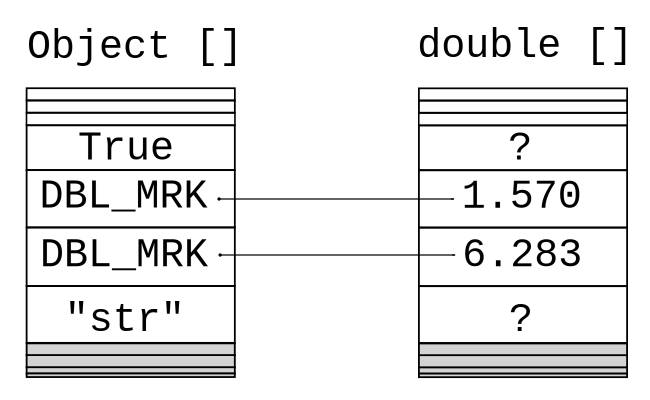
\includegraphics{fig/rhino_stack.pdf}
    }
    \caption{Znázornění koexistence hlavního a číselného zásobníku}
    \label{Figure.RhinoStack}
  \end{center}
\end{figure}

Interpret JavaScriptu přijímá mezikód jazyka, který je generován metodou compile třídy \texttt{CodeGenerator}. Generátor mezikódu pracuje s abstraktním syntaktickým stromem tvořeným z prvků definovaných v balíku \texttt{org.mozilla.JavaScript.ast} a generovaným třídou \texttt{Parser}.

\section{Nashorn}
\label{Chapter.JavaScriptInJavaAnalysis.Nashorn}

Nashorn je projekt, který si klade za cíl vyvinout zcela nový, odlehčený a výkonný JavaScriptový runtime pro nativní JVM. Výstupem projektu by měla být schopnost spouštět JavaScriptový kód příkazem jrunscript, která podléhá specifikaci JSR 223\footnote{JSR 223 -- specifikace definující framework pro vkládání skriptů do zdrojového kódu Javy}. Oproti poměrně letitému JavaScriptovému interpretu Rhina vyvinutému pro tehdejší JVM, se Nashorn zaměřuje na nové techniky používání dynamických jazyků v~Javě a vychází ze specifikace \linebreak tzv. Da Vinci stroje (JSR 292\footnote{JSR 292 -- specifikace pro rozšíření JVM o nativní podporu dynamických jazyků}). \cite{Bibliography.Nashorn.Project}

Jádro interpretu Nashorn vychází z ECMAScriptu verze 5.1. Skripty jazyka JavaScript lze v~Javě vytvářet užitím klasického Java API pro skriptování popsaného blíže v kapitole \ref{Chapter.JavaScriptInJavaAnalysis.ScriptingJavaAPI}. Konkrétní instanci JavaScriptového jádra \texttt{ScriptEngine} získáme vyhledáním odpovídajícího slova např. „nashorn“ v továrně \texttt{ScriptEngineManager}. Naopak pokud chceme spustit JavaScriptový skript, můžeme toho dosáhnout příkazem jrunscript a specifikací skriptovacího jazyka přepínačem \texttt{-l}, předáním skriptu přepínačem \texttt{-e}, nebo souboru se skriptem přepínačem \texttt{-f}.

\section{Skriptovací Java API}
\label{Chapter.JavaScriptInJavaAnalysis.ScriptingJavaAPI}

V Javě byly postupem času implementovány všechny nejznámější skriptovací jazyky používající různá a vlastní rozhraní. To bylo základním podmětem pro vytvoření obecného a přenositelného skriptovacího Java API, které umožňuje propojit skripty s aplikací Javy. API muselo být napsáno velmi abstraktně, aby bylo aplikovatelné na jakýkoliv rozmanitý skriptovací stroj, ale zároveň muselo zahrnout všechny specifické aspekty známých skriptovacích jazyků. \cite{Bibliography.JavaAPI.Script.Book}

Skriptovací Java API vychází ze specifikace JSR 223. Tato specifikace definuje standardní framework a API pro tvorbu skriptu a jejich vkládání do Javovských aplikací. Specifikace ovšem nedefinuje jaký jazyk pro skriptování musíme zvolit. Proto můžeme použít pro skriptování jakýkoliv jazyk, který je kompatibilní s JSR 223. Použitím standardního API máme možnost psát skripty kompatibilní s JSR 223. A naopak při psaní skriptu, který je kompatibilní s JSR 223, máme garantováno, že budeme mít přístup k jakékoliv standardní Java knihovně.

Implementace Java API v JDK od Oraclu vychází z frameworku BSF \cite{Bibliography.BSF.Framework}. Tento framework byl vyvinut firmou IBM a ve verzi 2.x poskytoval základní množinu tříd umožňujících podporu skriptovacích jazyků v aplikacích Javy. S příchodem skriptovacího Java API byl vydán BSF framework verze 3.x, který se poté stal součástí zmíněného JDK.

Základní Oracle implementace JDK 6 a 7 skriptovacího API obsahuje upravený již zmíněný JavaScriptový stroj vycházející z knihovny Rhina. Zahrnutá Oracle verze knihovny Rhina byla omezena o některé vlastnosti, které by poskytovalo přímé použití knihovny. Z důvodu bezpečnosti byl zakázán kompilátor do mezikódu Javy. V JDK nelze najít ani pomocné nástroje příkazové řádky distribuované Rhinem od Mozilly, jako jsou např.: JavaScriptový shell, debugger apod. Použitá implementace Rhina umožňovala definovat abstraktní třídy a implementovat vícenásobná rozhraní pomocí adaptéru JavaAdapter. Oracle nahradil tento adaptér vlastní třídou, která umožňuje implementaci pouze jednoduchých rozhraní. 

\subsection{Architektura skriptování}
\label{Chapter.JavaScriptInJavaAnalysis.ScriptingJavaAPI.ArchitectureOfScripting}

\bigskip \noindent Skriptovací API je umístěné v balíčku \texttt{javax.script}. Skriptování je poměrně přímočaré. Abychom mohli začít psát skripty, vždycky nejprve musíme:

\begin{enumerate}
  \item Vytvořit objekt třídy \texttt{ScriptEngineMager} -- objekt vyhledává skriptovací enginy \texttt{ScriptEngine} v načtených JAR knihovnách, je to tzv. továrna na skriptovací enginy;
  \item Získat instanci skriptovacího enginu \texttt{ScriptEngine} -- instance skriptovacího enginu je získána z továrny zavoláním např. metody \texttt{getEngineByName()}. 
\end{enumerate}

Jakmile máme získanou instanci skriptovacího enginu, můžeme již vykonávat, definovat, nebo upravovat skripty.

Nejdůležitější metodou rozhraní \texttt{ScriptEngine} je bezpochyby metoda \texttt{eval()}, která nám umožní spouštět skripty. Skript může být předán jako řetězec, nebo může být umístěn v~souboru, streamu, či jiném zdroji. V závislosti na tom, zda daný skriptovací jazyk umožnuje vyhodnocování skriptu s výsledkem, tak je metoda \texttt{eval()} vrácí i výsledek skriptu.

Myšlenkou Java API je mít co nejvíce společných rysů skriptovacích jazyků specifikovaných v rozhraní \texttt{ScriptEngine} a nemít zde žádný rys, který by některý skriptovací jazyk nemohl poskytnout. Proto všechny speciální vlastnosti konkrétních skriptovacích jazyků musí být implementovány v odlišných rozhraních. Tento návrh zajišťuje minimum změn těchto rozhraní v budoucnu. 

\bigskip \noindent Nejdůležitější přídavnými rozhraními rozpoznáváme:

\begin{itemize}
  \item \textbf{\texttt{Invocable}} -- rozhraní implementované enginy, které umožňují volat funkce/metody ve skriptu. Pro volání funkce používáme \texttt{invokeFunction()}, pro metody invokeMethod();
  \item \textbf{\texttt{Compilable}} -- rozhraní implementované enginy, které jsou schopny kompilovat skript do svého mezikódu.
\end{itemize}

\subsection{Data binding}
\label{Chapter.JavaScriptInJavaAnalysis.ScriptingJavaAPI.DataBinding}

Důležitým úkolem pro funkci frameworku Java API, je zajistit sdílení dat mezi hostovanou aplikací Javy a skriptovacím strojem. Framework BSF umožňoval sdílení proměnných pouze po náležité registraci v manažeru skriptovacích enginů, k němuž měly přístup všechny skriptovací enginy. Java API model data bindingu dále vylepšuje tím, že udržuje sdílené proměnné pomocí kontextu, ve kterém je skript spouštěn.

Proměnné jsou seskupeny a uloženy ve jmenných prostorech neboli scopech. Abstrakce uchovávání proměnných ve scopu je dána rozhraním \texttt{javax.script.Bindings}, přičemž se nejedná o nic jiného, než o jednoduché mapování názvu proměnné na náležitý objekt -- \texttt{Map<String, Object>}. Každý kontext skriptu obsahuje právě množinu takovýchto jmenných prostorů.

\bigskip \noindent Specifikace uvádí dva základní jmenné prostory:

\begin{itemize}
  \item \textbf{Enginový scope} -- proměnné, které se vážou k tomuto scopu nejsou viditelné jiným strojem;
  \item \textbf{Globání scope} -- ke všem proměnným tohoto scopu mají přístup všechny enginy vytvořené danou instancí enginového manažeru.
\end{itemize}

Pokud chceme vytvořit novou proměnnou, dosáhneme toho zavoláním metody \texttt{put()} objektu \texttt{Bindings}. Proměnnou v enginovém scopu lze definovat následovně:

\begin{enumerate}
  \item Nastavením vlastního objektu \texttt{Bindings} -- vytvořit mapovací objekt Bindings, kde vytvoříme naši proměnnou. Tento mapovací objekt nastavíme v enginu buď metodou \texttt{setBindings()}, nebo případně až za běhu skriptu parametrem v metodě \texttt{eval()};
  \item Využitím enginového objektu \texttt{Bindings} -- získáme výchozí mapovací objekt enginu metodou \texttt{getBindings()}, do kterého následně vložíme naši proměnnou.
\end{enumerate}

Získání hodnoty proměnné se docílí obdobně pouze metodou \texttt{get()}.

Základní vlastností frameworku je uchovávání stavu proměnných po vykonání skriptu. Všechny proměnné, které jsou ve skriptu inicializovány, se také automaticky vloží do odpovídajícího objektu \texttt{Bindings}. Po skončení skriptu jsou vytvořené proměnné dostupné v~odpovídajícím scopu, kde byly vytvořeny. Tento stav scopu zůstává i do dalšího vyhodnocení metodou \texttt{eval()}.

Jmenné prostory jsou pouze jedním stavebním prvkem třídy \texttt{SimpleScriptContext} -- kontextu skriptu. Všechny stavové objekty, které jsou pro běh skriptu podstatné, jsou uložené právě v této třídě. Dokonce i výše popsaný globální a enginový scope je uchováván zde. Jmenné prostory jsou zde uloženy ve formě listu čísel, které identifikují jednotlivé scopy. Čísla ve skutečnosti představují prioritu scopu. Nízká čísla popisují scopy s vysokou prioritou a vysoká čísla s nízkou prioritou. Ve vyhodnocování skriptu to znamená, že pokud např. hledáme proměnnou, která je ve dvou scopech zároveň, tak bude navrácena pouze ta proměnná ze scopu, který má vyšší prioritu. Enginovému scopu je přiřazena priorita 100, globálnímu scopu priorita 200. Kromě dvou základních scopů si můžeme definovat i vlastní jmenný prostor. Pro vytvoření vlastního jmenného prostoru ovšem nestačí nastavit tento scope pomocí \texttt{setBindings()} ve třídě \texttt{SimpleScriptContext}, protože třída přijímá pouze dva základní kontexty. Proto musíme definovat svůj vlastní kontext implementující rozhraní \texttt{ScriptContext}.

\chapter{Návrh}
\label{Chapter.Design}

Dle zadání této práce máme implementovat podporu pro klientský JavaScript do experimentálního vykreslovacího stroje CSSBox napsaném v jazyku Java. Výsledná aplikace by měla být opět psána v čistém jazyce Java bez použití nativních knihoven, tudíž by neměla narušovat přenositelnost stroje CSSBox.

Z  analýzy problematiky jednotlivých existujících strojů JavaScriptu v jazyce Java víme, že v současné době nemáme příliš mnoho na výběr. Jediným použitelným řešením pro skriptování, zejména z důvodu podpory hostování objektů Javy ve skriptech JavaScriptu, je pouze knihovna Rhino. Aby se v budoucnu ovšem dalo lehce přejít případně na jiný JavaScriptový stroj, budeme pro implementaci podpory klientského JavaScriptu používat a skriptování z jazyka Javy výhradně standardní skriptovací Java API.

V návrhu se konkrétně zaměříme na problematiku zpracování skriptů z HTML dokumentu (kapitola \ref{Chapter.Design.ScriptsInHTML}) a uvedeme možnost jak zařadit podporu pro skriptování do projektu SwingBox (viz kapitola \ref{Chapter.Design.ScriptsInSwingBox}). V kapitole \ref{Chapter.Design.GlobalScopeInjections} naznačíme techniku automatických instalací rozšíření do hlavního scopu JavaScriptu. Kapitola \ref{Chapter.Design.JavaScriptEngineJSR223} se bude zabývat spíše experimentální problematikou a to implementací základního zabezpečení do skriptovacího stroje Rhino. V závěru návrhu (kapitola \ref{Chapter.Design.SwingBoxIntegration}) budeme demonstrovat integraci rozšíření klientského JavaScriptu do projektu SwingBox.

Návrh byl proveden s ohledem na již existující třídy projektu CSSBox a ostatních knihoven. Návrh vychází z veřejných rozhraní tříd a není-li to zapotřebí, tak se nesnaží již existující třídy znovu implementovat. 

\bigskip \noindent Očekávanými závislostmi projektu budou knihovny a projekty:

\begin{itemize}
  \item \textbf{CSSBox} \cite{Bibliography.CSSBox} -- (X)HTML renderovací knihovna,
  \item \textbf{CSSParser} \cite{Bibliography.jStyleParser} -- parser kaskádových stylů,
  \item \textbf{SwingBox} \cite{Bibliography.SwingBox} -- prohlížeč webových stránek využívající CSSBox,
  \item \textbf{Rhino} \cite{Bibliography.Rhino.Docs} -- skriptovací stroj JavaScriptu,
  \item \textbf{Google Juice} \cite{Bibliography.Google.Juice} -- pro umožňění injektáže závislostí (angl. dependency injection),  
  \item \textbf{NekoHTML} \cite{Bibliography.NekoHTML} -- parser HTML dokumentu,
  \item \textbf{Apache CXF} \cite{Bibliography.Apache.CXF} -- knihovna klient/server služeb.
\end{itemize}

Projekt bude vyvíjen na systému Windows 8 v prostředí Eclipse s JDK 1.7.0\_25. Za cíl si projekt klade poskytnout zpětnou podporu pro JRE/JDK 6.
 
\section{Provádění skriptů v HTML dokumentu}
\label{Chapter.Design.ScriptsInHTML}

Klientské skripty jsou v HTML dokumentu specifikovány elementy \texttt{<script>}. Jak bylo uvedené v kapitole \ref{Chapter.DependenciesAnalysis.ScriptsInHTML}, lze skripty vykovávat ihned po dokončení parsování značky se skriptem a nemusí se čekat, dokud je celý dokument načten. 

V současné době není v~rámci projektu CSSBox podpora pro manipulaci s dokumentem, který je právě čten. Aby bylo možné implementovat podporu pro skriptování přesně podle HTML specifikace, budeme muset implementovat vlastní parser dokumentu. Základní navrženou techniku implementace parseru dokumentu lze spatřit na obrázku \ref{Figure.EventDOMParserDesign}.

\begin{figure}[H]
  \begin{center}
    \scalebox{0.65}{
      \includegraphics{fig/org-fit-cssbox-jse-document.pdf}
    }
    \caption{Diagram tříd parseru dokumentu \texttt{EventDOMParser}}
    \label{Figure.EventDOMParserDesign}
  \end{center}
\end{figure}

Podle návrhu bude nutno definovat vlastní parser \texttt{EventDOMParser}, který vychází z parseru \texttt{DOMParser} knihovny NekoHTML. Tento parser bude průběžně zpracovávat vstupní dokument a informovat o aktuálním stavu parsování pomocí speciálních událostí. Události budou nést informaci, zda bylo zahájeno či ukončeno parsování určitého uzlu. Pokud parsování bylo dokončeno, bude si moci naslouchající objekt vyzvednout rozparsovaný uzel. 

Knihovní třída \texttt{DOMParser} využívá pro vytváření dokumentu implementované rozhraní \texttt{XMLDocumentHandler}, které obsahuje obslužné metody informující o stavu parsování. V~rámci těchto obslužných metod dochází k vytváření jednotlivých uzlů dokumentu a konstruování výsledného stromu dokumentu. Současnou implementaci objektu, který zajišťuje konstrukci stromu dokumentu lze získat z konfigurace parseru.

Odchytávání událostí během parsování bude umožněno přenastavením aktuální implementace instance třídy \texttt{XMLDocumenthandler} v konfiguraci parseru \texttt{DOMParser}. Naším cílem bude v rámci volání obslužných metod zavolat i naši vlastní událost. Abychom ovšem nemuseli předefinovat celou funkčnost konstrukce dokumentu, budeme využívat starý knihovní \texttt{XMLDocumentHandler} získaný z konfigurace. Upravený \texttt{EventXMLDocumentHandler} bude knihovní handler pouze dekorovat a zajišťovat propagaci některých události výše do třídy \texttt{EventDOMParser}. 

Aby byl návrh kompletní, byla navržena i třída \texttt{NodeEventDispatcher} vykonávající události \texttt{NodeEvent}. Všichni zájemci o naslouchání událostí si budou muset zaregistrovat naslouchající objekt ve třídě \texttt{EventDOMParser}, který dále tento objekt zaregistruje i ve třídě \texttt{NodeEventDispatcher}. Objekty odchytávající události parseru budou implementovat rozhraní \texttt{NodeEventListener} vycházející ze standardního rozhraní Javy \texttt{EventListener}.

\section{Podpora skriptování v projektu SwingBox}
\label{Chapter.Design.ScriptsInSwingBox}

Jak bylo popsáno v kapitole \ref{Chapter.DependenciesAnalysis.SwingBox}, projekt SwingBox umožňuje zobrazovat a procházet webové stránky. Pro přidání podpory skriptování do tohoto projektu (viz kapitola \ref{Chapter.Design.SwingBoxIntegration}) bude nutno definovat vlastní třídu \texttt{CSSBoxAnalyzer}. SwingBox používá tuto třídu pro parsování vstupního dokumentu a převod dokumentu na vykreslovaný \texttt{ElementBox}.   

\begin{figure}[H]
  \begin{center}
    \scalebox{0.75}{
      \includegraphics{fig/org-fit-cssbox-jse-util.pdf}
    }
    \caption{Diagram tříd znázorňující podporu JavaScriptu v projektu SwingBox}
    \label{Figure.ScriptsInSwingBoxDesign}
  \end{center}
\end{figure}

Projekt \texttt{CSSBox} definuje pro zdroj dokumentu třídu \texttt{DocumentSource}, pro čtení dokumentu ze zdroje dokumentu třídu \texttt{DOMSource}. Abychom jsme se drželi zavedené praktiky pro čtení dokumentu s událostmi, v návrhu definujeme třídu \texttt{EventDOMSource}, která pouze vnitřně používá v kapitole \ref{Chapter.Design.ScriptsInHTML} popsaný \texttt{EventDOMParser}. 

Největší roli při invokaci skriptu hraje v návrhu \texttt{ScriptAnalyzer}, který má u událostního parseru zaregistrovaný vlastní \texttt{EventNodeListener}. Při příchodu události o zpracování elementu \texttt{<script>}, přečte \texttt{ScriptAnalyzer} skript v jeho těle, případně načte skript z URL adresy uvedené v \texttt{src} atributu. Pokud skript neobsahoval atribut \texttt{defer}, tak se dále nechá ihned vykonávat ve stroji \texttt{DocumentScriptEngine}. Stroj, který má být použit pro aktuální skript je získán z instance třídy \texttt{DocumentScriptManager} na základě atributu \texttt{type} elementu \texttt{<script>}, nebo z výchozího uvedeného stroje v \texttt{<meta>} značce (viz kapitola \ref{Chapter.DependenciesAnalysis.ScriptsInHTML}).

\begin{figure}[H]
  \begin{center}
    \scalebox{0.55}{
      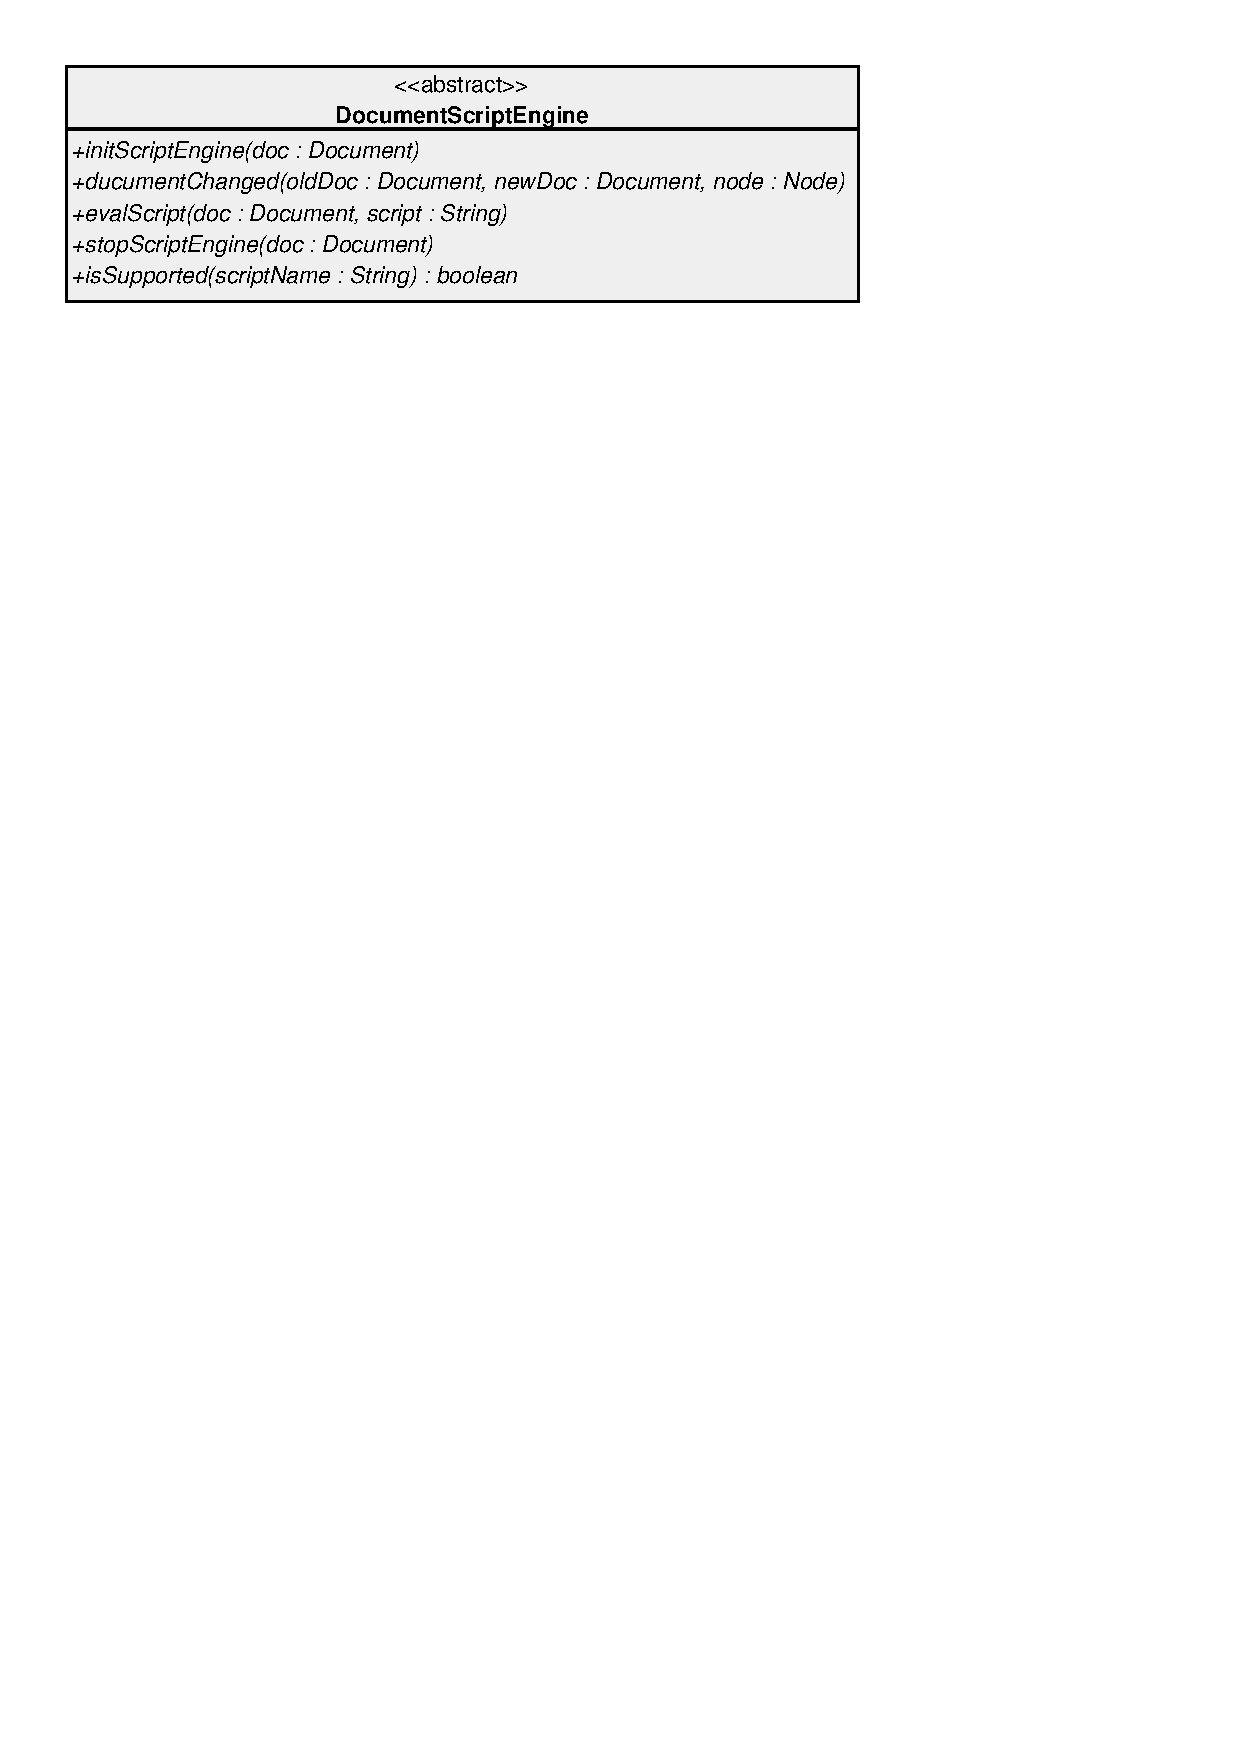
\includegraphics{fig/javascsript-engine.pdf}
    }
    \caption{Diagram abstraktní třídy \texttt{DocumentScriptEngine}}
    \label{Figure.DocumentScriptEngineDesign}
  \end{center}
\end{figure}

Pokud je skript vykováván poprvé v rámci uvedeného dokumentu, tak dojde u třídy \texttt{DocumentScriptEngine} (obrázek \ref{Figure.DocumentScriptEngineDesign}) i k zavolání metody \texttt{initScriptEngine()}, která vytvoří globální scope pro vykonávání skriptů. V globální scopu jsou poté vykonávány všechny skripty na stránce. Skriptovací stroj uchovává jednotlivé zaregistrované dokumenty a jejich vykonávací globální scopy dokud není webová stránka přenačtena a dokument není změněn. O zničení dokumentu bude stroj informován metodou \texttt{stopScriptEngine()}.

\section{Injektování objektů do hlavního scopu}
\label{Chapter.Design.GlobalScopeInjections}

Během implementace podpory klientského JavaScriptu do projektu CSSBox se předpokládá vytvoření velké množství tříd, které budou implementovat jednotlivé aspekty JavaScriptu pro prohlížeč. Předpokládá se, že vyvíjené třídy budou vyvíjeny postupně a iterativně přidávat jednotlivé funkčnosti. Bylo by výhodné oddělit jednotlivé nové funkce a odstranit potřebu přímého zásahu do třídy \texttt{DocumentScriptEngine} s příchodem nového rozšíření. 

\begin{figure}[H]
  \begin{center}
    \scalebox{0.75}{
      \includegraphics{fig/org-fit-cssbox-jse-script-inject.pdf}
    }
    \caption{Diagram tříd znázorňující podporu injektování rozšíření JavaScriptu}
    \label{Figure.GlobalScopeInjectionsDesign}
  \end{center}
\end{figure}

K separaci nových implementovaných vlastností JavaScriptu byla navržena technika injekce funkčnosti do vytvořeného kontextu (obrázek \ref{Figure.GlobalScopeInjectionsDesign}). Pro přidání nové funkčnosti do globálního scopu kontextu bude nutno implementovat abstraktní třídu \texttt{ScriptContextInject}. Samotnou injekci do globálního scopu bude provádět metoda \texttt{inject()}. Aby skriptovací stroj věděl, jaká rozšíření má injektovat do svého scopu, měla by být jednotlivá rozšíření registrována u skriptovacího stroje metodou \texttt{installContextInject()}. Injekce bude prováděna vždy po vyhodnocení některého skriptu, nebo po inicializování nového dokumentu. Pořadí jednotlivých injekcí bude v základní implementaci určovat metoda \texttt{getPriority()}. Zda je injekce validní, tudíž proveditelná, bude získáváno metodou \texttt{isValid()}. Příkladem, kdy injekce by byla neproveditelná, by mohla být např. situace, kdy není ještě dokument úplně načten a některé rozšíření by záviselo právě na existenci dokumentu.

Neustálá instalace nové injekce rozšíření do skriptovacího stroje s příchodem nového rozšíření by se postupem času nejevila jako dobré řešení. Bylo by výhodné, aby s novým rozšířením došlo i k automatické instalaci tohoto rozšíření do skriptovacího stroje, tzn., abychom dosáhli obrácení řízení -- IoC (Inversion of Control). Pro tento účel byla navržena třída \texttt{ScriptContextInjector}, která kromě metod samotné injekce bude provádět i registraci rozšíření v odpovídajícím skriptovacím stroji. K získání reference registru skriptovacích strojů \texttt{DocumentScriptManager} z objektů ScriptContextInjector se bude používat injektáž závislosti -- DI (Dependency Injection). Pro podporu DI je v plánu použít knihovnu Google Juice. Ve třídě \texttt{ScriptContextInjector} se v závislosti na typu skriptu vyhledá v registru skriptovacích strojů odpovídající stroj, ve kterém proběhne registrace samotné injekce rozšíření. 

Pokud celý návrh injektování shrneme, tak automatická registrace injekce rozšíření bude probíhat v abstraktní třídě \texttt{ScriptContextInjector}. O tom, do jakého skriptovacího stroje by se měla injekce rozšíření vložit, bude informovat pro jazyk JavaScript např. třída injektoru \texttt{JavaScriptContextInjector}. Samotná injekce rozšíření bude přitom implementována až specifickými injektory, jako jsou např. \texttt{DocumentInjector}, \texttt{HistoryInjector}, apod.

\section{Implementace stroje JavaScriptu podle normy JSR 223}
\label{Chapter.Design.JavaScriptEngineJSR223}

Poslední iterací v integraci JavaScriptového stroje do projektu CSSBox by bylo přizpůsobit skriptovací stroj tak, aby splňoval bezpečnostní předpoklady pro běh v prohlížeči. Budeme muset zabránit zejména přístupu do tříd a balíků Javy, které nenesou žádnou funkční hodnotu pro implementaci klientského JavaScriptu. Z důvodu snazšího přechodu na jiný skriptovací stroj, např. Nashorn, by bylo výhodné, aby byl stroj implementován podle standardu JSR 223. Nashorn je vyvíjen se standardním rozhraním již od základu.

Pro tvorbu takového stroje by se nabízelo využít již existující stroj implementovaný v~Java API, který se nachází v balíku sun.org.mozilla.JavaScript. Třídy Java API jsou ovšem finální, nebo skryty, což brání jejich znovupoužití. Nezbývá nám než implementovat vlastní skriptovací stroj, který rozšiřuje základní třídu pro skriptovací stroje AbstractScriptEngine. Tento stroj bude pro implementaci samotného skriptování využívat externí knihovnu Rhino. Rozhodnutí pro dodání externí knihovny bylo učiněno z důvodu, abychom nebyli závislí na knihovně, která je dodávaná v JDK v balíku \texttt{sun.org.mozilla.JavaScript.internal}. Osamostatněním na implementaci JDK získáme kompletní správu nad verzí knihovny a nebudeme muset řešit případné problémy s příchodem JDK 8, kde již Rhino zřejmě nebude ani v rámci základní distribuce JDK.

Způsob, kterým by mohl být implementován JavaScriptový stroj s implementovanými bezpečnostními funkcemi je navržen na obrázku \ref{Figure.JavaScriptEngineJSR223Design}:

\begin{figure}[H]
  \begin{center}
    \scalebox{0.80}{
      \includegraphics{fig/org-fit-cssbox-jse-script.pdf}
    }
    \caption{Diagram tříd zabezpečeného skriptavacího stroje JavaScriptu}
    \label{Figure.JavaScriptEngineJSR223Design}
  \end{center}
\end{figure}

Skriptovací stroj spravující jednotlivé načtené webové dokumenty reprezentovaný třídou \texttt{JavaScriptDocumentEngine} bude používat instanci námi upraveného skriptovacího stroje nazvaného \texttt{RestrictedRhinoScriptEngine}. Aby byla splněna specifikace JSR 223, tak bude tento stroj vytvářen pomocí továrny, která bude realizovat abstraktní třídu Java API \texttt{ScriptEngineFactoryBase}. Třída \texttt{RestrictedRhinoScriptEngine} bude muset implementovat abstraktní třídu pro všechny skriptovací stroje \texttt{AbstractScriptEngine}. Jelikož JavaScript umožňuje i volat funkce, tak bude dodatečně implementováno i rozhraní \texttt{Invocable}. 

Námi implementovaný stroj bude staticky vytvářet objekty nejvyšší úrovně a standardní objekty JavaScriptu, které budou společné pro globální scope a pro každé vykonávání skriptu. Staticky bude vytvořena i továrna \texttt{JavaShutterContextFactory} pro vytváření kontextu, která implementuje \texttt{ContextFactory}. Továrna je automaticky volána knihovnou Rhino pokaždé, když vstoupíme do nového kontextu metodou \texttt{Context.enter()}. Továrna kontextu bude instalovat do kontextu vlastní obalující továrnu \texttt{ShutterWrapFactory} a objekt třídy \texttt{JavaShutter} sloužící pro omezení přístupu do jazyka Javy. Objekt omezující bezpečnost bude viditelný i z továrny pro obalování objektů Javy.

Důvodem pro předefinování továrny obalující objekty, která je volána pro každou třídu, objekt, metodu, primitivní typ Javy použitý v kódu JavaScriptu, je právě přidání podpory rozmělnění bezpečnosti. Samotným účelem obalující továrny je dodání rozhraní \texttt{Scriptable} do objektů Javy, tak aby byly viditelné z kódu JavaScriptu. Ve vlastní implementaci továrny budeme provádět před obalením položky ověření, zda je položka viditelná. Pokud položka nemá být viditelná, tak nedojde k požadovanému obalení položky, takže položka z kódu JavaScriptu nebude viditelná.

Knihovna Rhino již obsahuje rozhraní \texttt{ClassShutter} pro zajištění bezpečnosti přístupu do Javy. Rozhraní \texttt{ClassShutter} však obsahuje pouze jednu metodu, která ověří, zda je požadovaná třída viditelná. Navrhnutá architektura na obrázku \ref{Figure.JavaScriptEngineJSR223Design} ovšem uvádí rozmělnění zabezpečení do menších položek, jako jsou povolené metody, atributy aj. Takovéto rozmělnění bude zajištěno objektem \texttt{JavaShutter}, který bude poskytovat informaci o tom, zda je přistupovaná třída, metoda, vlastnost apod. viditelná z kódu JavaScriptu. Registrace viditelných položek bude implementačně prováděna manuálně zavoláním určité metody nad objektem \texttt{JavaShutter}. Budeme mít ale i možnost nechat viditelnost odvodit automaticky podle anotace položky. Pro viditelné položky Javy zavedeme vlastní anotaci \texttt{@JSVisible}. 

Druhým bezpečnostním omezením bude omezení adaptéru zabezpečujícího implementaci rozhraní a abstraktních tříd Javy -- \texttt{JavaAdapter}. Předpokládá se, že tato funkčnost bude kompletně zakázána.

Po vyřešení bezpečnosti budeme muset implementovat samotné propojení rozhraní Rhina a specifikace JSR 223. Důležité bude vyřešit data binding pro kontext \texttt{ScriptContext} definovaný v této specifikaci. Abychom měli přehled o všech proměnných, které se ve hlavním scopu nachází, budeme muset vytvořit třídu vlastního scopu. Scope (viz kapitola \ref{Chapter.JavaScriptInJavaAnalysis.Rhino.ScriptingWithRhino}) je klasický JavaScriptový objekt, ve kterém probíhá spouštění skriptu, tudíž implementuje rozhraní \texttt{Scriptable}. Rozhraní specifikuje metody pro zápis \texttt{put()} a získání atributů \texttt{get()} z objektu. Tyto metody jsou během vykonávání skriptu náležitě volány. Zpětného volání metod využijeme k navázání atributů do objektu \texttt{Bindings} a nebo získání atributů z objektu \texttt{Bindings}. 

Výše popsané praktiky jsou dostatečné pro vytvoření jednoduchého stroje, který vychází ze specifikace JSR 223.  Po zavolání vykonání skriptu metodou \texttt{eval()}, bude pracovat stroj tak, jak je popsáno v následujících krocích:  

\begin{enumerate}
  \item	Vytvoří se nový kontext zavoláním \texttt{Context.enter()}, v rámci něhož dojde i k zavolání metody \texttt{makeContext()} třídy \texttt{JavaShutterContextFactory};
  \item	Vytvoří se nový hlavní scope, který bude nastavovat a číst \texttt{Bindings} objekt;
  \item	Do hlavního scopu se vloží standardní a globální objekty, které budou společné pro všechny skripty. Vložení proběhne nastavením prototypu hlavního scopu;
  \item	Spustí se skript nad vytvořeným kontextem a hlavním scopem.
\end{enumerate}

\section{Integrace podpory JavaScriptu do SwingBoxu}
\label{Chapter.Design.SwingBoxIntegration}

Všechny potřebné náležitosti pro zařazení podpory JavaScriptu do projektu CSSBox byly již navrženy. Návrh proběhl konkrétně pro podprojekt SwingBox, který rozšiřuje výchozí  CSSBox o reakci prvků stránky na podněty příchozí od uživatele, tzn. zejména o možnost procházení webového obsahu. 

Aby bylo možné zakomponovat JavaScript do projektu SwingBox, bude nutno provést registraci vlastní \texttt{CSSBoxAnalyzer} třídy navržené v kapitole \ref{Chapter.Design.ScriptsInSwingBox}. Kompletní konfigurace, kterou bude nutno provést pro přidání podpory JavaScriptu je znázorněna na obrázku \ref{Figure.SwingBoxIntegrationDesign}.

\begin{figure}[H]
  \begin{center}
    \scalebox{0.80}{
      \includegraphics{fig/swingbox-integration.pdf}
    }
    \caption{Sekvenční diagram znázorňující kroky integrace JavaScriptového stroje}
    \label{Figure.SwingBoxIntegrationDesign}
  \end{center}
\end{figure}

Z uvedeného diagramu je patrné, že pouhá jedna registrace vlastního vyhodnocovače dokumentu \texttt{ScriptAnalyzer} bude pro přidání podpory JavaScriptu dostačující. Projekt SwingBox zejména implementuje vlastní zobrazovací plochu pro webové stránky \texttt{BrowserPane}. Zobrazovací plochu využijeme ve finální čísti projektu pro tvorbu jednoduchého webového prohlížeče a znázornění funkčnosti skriptování v HTML dokumentech. Třída pro zobrazování obsahu HTML stránky využívá pro veškeré čtení nového dokumentu webové stránky třídu \texttt{SwingBoxEditrKit}, která následně volá \texttt{ContentReader}, jenž je přímo spjat s~aktuálně zaregistrovaným \texttt{CSSBoxAnalyzer}. Definicí vlastní třídy \texttt{ScriptAnalyzer} získáme plnou kontrolu nad zpracovávaným dokumentem a možnost provádění skriptů v HTML dokumentu. 

\chapter{Závěr}
\label{Chapter.Final}

Cílem této práce bylo se seznámit s projektem CSSBox a zanalyzovat problematiku skriptování v jazyce JavaScript z jazyka Javy. Na základě získaných teoretických znalostí navrhnout architekturu a způsob integrace skriptovacího stroje do projektu CSSBox.

V rámci práce bylo nejprve analyzováno skriptování v HTML dokumentech a referenční způsob pro přidání skriptovací podpory do dokumentu. Byl představen projekt CSSBox, do kterého bude integrování rozšíření probíhat a komponenta SwingBox pro zobrazování HTML dokumentu.

V kapitole analýzy skriptovacích strojů byly demonstrovány existující řešení pro skriptování v jazyce JavaScript v Javovských aplikacích. Podrobně byla rozebrána technika tvorby skriptů s API knihovny Rhino. V kontrastu na tvoru skriptů s nestandardním API Rhina, byla ukázána i tvorba skriptu se standardním skriptovacím API Javy.

Návrh integrace rozšíření skriptování v JavaScriptu přímo reflektoval teoretickou analýzu z předešlých kapitol. Z důvodu asynchronního spouštění skriptů jsme museli navrhnout inkrementální načítání dokumentu. Abychom odstranili potřebu měnit kód skriptovacího stroje při přidávání nového rozšíření hlavního scopu, jsme navrhli injektování do skriptovacího stroje s využitím injektáže závislostí. Jelikož knihovna Rhino obsahovala pouze základní kontrolu přístupu do Javy z JavaScriptu, navrhli jsme také třídy pro rozmělnění bezpečnosti a lepší správu bezpečnostních politik. Závěrem návrhu jsme demonstrovali příklad „registrace“ samotného rozšíření do projektu SwingBox.
